\documentclass[a4paper, 14pt]{extreport}
% !TeX spellcheck = ru_RU
%Автор - Краснов Александр 2022

%Настройка языка и отображения
\usepackage[russian]{babel}
%Шрифты
\usepackage[T2A]{fontenc}		%Русские шрифты
%\usefont{T2A}{Tempora-TLF}{m}{n}
%\usepackage{lmodern}			%Шрифт Latin Modern, нужен если нет cm-super

\usepackage[utf8]{inputenc}		%Кодировка
\usepackage{amssymb,amsmath}	%Математические символы
\usepackage{multicol}			%Несколько колонок
%\usepackage{color}				%Использовать цветной текст

\usepackage{graphicx}			%Пикчи
\DeclareGraphicsExtensions{.pdf,.png,.jpg}
\frenchspacing					%Отключает большой пробел между предложениями

\usepackage{indentfirst}		%Красная строка
\setlength{\parindent}{1.25cm}	%Настройка отступа красной строки для шрифта 14pt, по умолчанию 15pt
\linespread{1.25} 				%Межстрочный интервал

\usepackage{parskip} 			%Интервал между абзацами
\setlength{\parindent}{1cm} 	%Настройка интервала между абзацами, по умолчанию будет 0

\usepackage{enumitem}			%Настройка списков
\setlist{noitemsep}				%Убирает лишнюю строку в списках

\usepackage{textcomp}			%Улучшает знак номера

\usepackage{cmap}				%Ссылки в PDF
\usepackage[					%Гипертекстовое оглавление в PDF
bookmarks=true, colorlinks=true, unicode=true,
urlcolor=black,linkcolor=black, anchorcolor=black,
citecolor=black, menucolor=black, filecolor=black,
]{hyperref}

%\sloppy						%Автоматическое разряжение строк (только для черновиков)
\emergencystretch=20pt			%Аварийное разряжение строк (подбор опытным путем)
%\hfuzz=0.5pt					%Разрешить переполнение абзаца на 0.5dd (выглядит приемлемо)
\tolerance=300					%Настройка максимальной разряженности строки
\hyphenpenalty=100				%Настройка частоты переносов

\clubpenalty=5000				%Настройка висячих строк в начале абзаца от 0 до 10000
\widowpenalty=5000				%настройка висячих строк в конце абзаца от 0 до 10000


%Колонтитулы и номера страниц
%\pagestyle{empty} 				%Нет ни колонтитулов, ни номеров страниц
\pagestyle{plain} 				%Номера страниц ставятся внизу в середине строки, колонтитулов нет
%\pagestyle{headings} 			%Присутствуют колонтитулы (включающие в себя и номера страниц)
%\pagestyle{myheadings}			%То же, что и headings, но делается вручную

\pagenumbering{arabic}			%Нумерация страниц арабскими цифрами
%\pagenumbering{roman}			%Нумерация страниц римскими строчными цифрами
%\pagenumbering{Roman}			%Нумерация страниц римскими заглавными цифрами
%\pagenumbering{alph}			%Нумерация страниц строчными английскими буквами
%\pagenumbering{Alph}			%Нумерация страниц заглавными английскими буквами
%\pagenumbering{asbuk}			%Нумерация страниц строчными русскими буквами
%\pagenumbering{Asbuk}			%Нумерация страниц заглавными русскими буквами


%\usepackage{fancyhdr}			%Колонтитулы
%\pagestyle{fancy} 				%Использование кастомных колонтитулов
%\fancyhf{} 					%Отчистить все колонтитулы
%\lhead{} 						% левый верхний колонтитул
%\chead{} 						% центральный верхний
%\rhead{} 						% правый верхний
%\lfoot{} 						% левый нижний
%\cfoot{\thepage} 				% центральный нижний
%\rfoot{} 						% правый нижний


\usepackage{listings}
% настройка подсветки кода и окружения для листингов
%\usemintedstyle{colorful}
%\newenvironment{code}{\captionsetup{type=listing}}{}


%Спецсимволы
\usepackage{wasysym}			%Специальные символы, в том числе и гачи
\newcommand{\gachi}{\male}		%Гачи значок


%реализовать модификаторы шрифтов горячими клавишами



%Настройки верстки
%\openany						%Глава может начинаться с любой страницы
%\openright						%Глава только с правой страницы

%\fleqn							%Формулы слева
%\leqno							%Номера формул слева

%\raggedbottom					%Страницы разной высоты
\flushbottom					%Страницы одинаковой высоты

%\columnseprule=0.4pt			%Ширина линейки при верстке в колонки
%\columnsep=0mm					%Расстояние между колонками при верстке в колонки


%Настройка страниц

\usepackage[left=1.5cm, right=1.5cm, top=1.5cm, bottom=1.5cm]{geometry}
%twoside, openany,%
\usepackage{pscyr}
\renewcommand{\rmdefault}{ftm}
\renewcommand{\ttdefault}{fcr}
\renewcommand{\sfdefault}{far}
% This package designed and commented in russian utf-8 encoding.
%
% Лицензия GNU GPL v2 и совместимые
%
% Автор - Алексей Томин, с помощью списка рассылки latex-gost-request@ice.ru
% Все вопросы, замечания и пожелания сюда: mailto:alxt@yandex.ru
%
% Дальнейшая разработка и поддержка - Михаил Конник,
% связаться можно по адресу mydebianblog@gmail.com
%
\ProvidesPackage{G7-32}[2003/07/07 v1.00 Titles for GOST 7.32-2001]

%стандартные части
\newcommand\Executors{%список исполнителей
 \chapter*{\CYRS\cyrp\cyri\cyrs\cyro\cyrk~%
           \cyri\cyrs\cyrp\cyro\cyrl\cyrn\cyri\cyrt\cyre\cyrl\cyre\cyr\cyrishrt}%
}
\newcommand\Referat{%реферат
 \chapter*{\CYRR\cyre\cyrf\cyre\cyrr\cyra\cyrt}%
}
\addto\captionsrussian{%содержание
 \def\contentsname{%
  \CYRS\cyro\cyrd\cyre\cyrr\cyrzh\cyra\cyrn\cyri\cyre}%
}
{}
\newcommand\NormRefs{%нормативные ссылки
 \chapter*{\CYRN\cyro\cyrr\cyrm\cyra\cyrt\cyri\cyrv\cyrn\cyrery\cyre~%
           \cyrs\cyrs\cyrery\cyrl\cyrk\cyri}%
}
\newcommand\Defines{%глоссарий
 \chapter*{\CYRG\cyrl\cyro\cyrs\cyrs\cyra\cyrr\cyri\cyrishrt}%
}
%\newcommand\Defines{%определения
% \chapter*{\CYRO\cyrp\cyrr\cyre\cyrd\cyre\cyrl\cyre\cyrn\cyri\cyrya}%
%}
\newcommand\Abbreviations{%обозначения и сокращения
 \chapter*{\CYRO\cyrb\cyro\cyrz\cyrn\cyra\cyrch\cyre\cyrn\cyri\cyrya~\cyri~%
           \cyrs\cyro\cyrk\cyrr\cyra\cyrshch\cyre\cyrn\cyri\cyrya}%
}
\newcommand\Introduction{%введение
 \chapter{\CYRV\cyrv\cyre\cyrd\cyre\cyrn\cyri\cyre}%
}
\newcommand\Conclusion{%заключение
 \chapter{\CYRZ\cyra\cyrk\cyrl\cyryu\cyrch\cyre\cyrn\cyri\cyre}%
}
\addto\captionsrussian{%список использованных источников
 \def\bibname{%
  \CYRS\cyrp\cyri\cyrs\cyro\cyrk~
  \cyri\cyrs\cyrp\cyro\cyrl\cyrsftsn\cyrz\cyro\cyrv\cyra\cyrn\cyrn\cyrery\cyrh~
  \cyri\cyrs\cyrt\cyro\cyrch\cyrn\cyri\cyrk\cyro\cyrv}%
}

\newcommand\NirTitle[1]{
 \thispagestyle{empty}
 \begin{centering}
  \linespread{1.1}\normalsize
  {\Nir@OrgLongName}

  \vfill

\Nir@AnnOtchet \Nir@Otchet

  \vspace{8mm}
  #1
  \vspace{8mm}

\Nir@StageNo~~\Nir@StageTitle

  \vfill
  \begin{tabular}{p{80mm}p{80mm}}
    \Nir@MainBegin, \newline
    \Nir@ManagerPost
   &
    ~\newline\underline{~~~~~~~~~~~~~~~~~~~} \Nir@ManagerName \newline
  \end{tabular}
  \vfill
  \vfill
  \Nir@Town~\Nir@Year

 \end{centering}
 \linespread{\Gost@LineSpread}\normalsize
}



%Словарь переносов
\hyphenation{
    про-из-вод-стве 
    до-пус-ти-мых 
    тех-но-ло-ги-чес-ких 
    рес-пи-ра-то-ров 
    про-вес-ти 
    э-лек-тро-маг-нит-но-го 
    ста-ти-сти-чес-ким 
    са-мо-сто-я-тель-но 
    ко-леб-лю-ще-го-ся 
    им-пульс-но-го 
    ус-та-нав-ли-ва-ют 
    не-пос-то-ян-но-го 
    ха-рак-те-рис-ти-ки
    про-из-вод-ствен-но-го 
    про-ме-жу-ток 
    пос-ле-ду-ю-щей
    раз-ве-ва-ю-щи-е-ся
    сви-са-ю-щи-е
    пред-ме-ты
    ре-зуль-та-те
    о-бес-то-чен
    за-кре-пи-те
    вни-ма-тель-ны
    и-зо-ля-ци-ю
    ком-плек-ту-ю-щи-е
    поз-во-ля-ет
    прак-ти-чес-ки
    об-ду-мать
    по-верх-нос-ти
    по-ло-же-ний
    по-лез-ность
    сто-ро-ной
    кон-струк-тив-но-го
    о-со-бен-нос-ти
    по-ни-ма-ния
    не-об-хо-ди-мые
    зна-ко-мых
    ис-поль-зу-ют-ся
    у-вле-ка-тель-ная
    ро-бо-то-тех-ни-ки
    у-прав-лять
    ин-струк-ци-ям
    у-да-лен-но
    функ-ци-о-наль-ность
    мо-ду-лю
    це-лом
    спе-ци-аль-нос-ти
    про-цесс
    об-щие
    по-лу-чи-ли
    ра-бо-та-ли
    тех-но-ло-ги-чес-кий
    ба-лан-си-ров-ки
    по-мощью
    ре-гу-ли-ру-ет-ся
    ско-рость
    от-но-си-тель-ную
    оп-ре-де-лять
    ком-пью-тер
    сиг-на-лы
    э-та-лон-ным
    пред-став-лен-но-го
    об-ра-зом
    пред-пи-сан-но-го
    пре-пят-ствий
    до-пол-ни-тель-ный
    преи-му-щест-ва
    кон-струк-ции
    за-клю-ча-ет-ся
    за-тра-ты
    на-мно-го
    сис-те-мах
    кон-ту-ру
    пе-ре-ход-ной
    ос-но-ве
    рас-сто-я-ние
    ос-лаб-ле-ние
    бла-го-да-ря
    за-мкну-то-му
    вы-со-кие
    ус-та-нов-ле-ния
    от-сле-жи-вать
    дат-чи-ка
    пред-став-лен-ный
    вклю-ча-ют
    по-мех
    от-ка-зов
    ис-поль-зо-ва-ние
    не-до-стат-ки
    на-прав-ле-ние
    от-ра-жа-тель-ной
    по-ло-же-ние
    раз-вер-нут
    сан-ти-мет-ры
    де-мон-стри-рует
    ин-же-нер-ных
    рас-счи-тан
    ба-лан-си-ру-ет
    сер-во-при-вод
    про-пор-ционал
    ал-го-ри-тм
    ко-то-рое
    по-ло-же-ния
    те-че-ни-ем
    по-лу-ча-ет
    сис-те-ма
    каж-дым
    уси-ле-ния
    ко-эф-фи-ци-ен-ты
    поль-зо-ва-те-лем
    ди-апа-зо-на
    от-но-си-тель-но
    зна-че-ния
    за-дан-но-го
    со-ед-и-не-нию
    дат-чи-ки
    вра-ще-ния
    из-ме-ря-ет
    ме-ха-ни-зма-ми
    ко-то-рый
    не-гра-ви-та-ци-он-ное
    прог-рам-ми-ро-ва-ние
    про-ф-ес-си-о-на-ль-ной
    де-я-т-е-ль-но-с-ти
    фор-ми-ро-ва-ние
    про-фес-сио-наль-ное
    ин-фор-ма-ции
    дея-тель-нос-ти
    до-к-у-м-ен-та-ц-ии
    при-ме-ни-тель-но
    об-о-р-у-до-ва-н-ия
    со-ци-аль-но-го
    не-об-хо-ди-мо-го
    го-су-дар-ст-вен-ном
    ис-поль-зо-вать
    сред-ст-ва
    фи-зи-чес-кой
    куль-ту-ры
    сох-ра-не-ния
    ук-р-е-п-л-е-н-ия
    про-цес-се
    под-дер-жа-ние
    не-об-хо-ди-мо-го
    фи-зи-чес-кой
    под-го-тов-лен-нос-ти
    вы-би-рать
    спо-со-бы
    ре-ше-ния
    про-фес-сио-наль-ной
    при-ме-ни-тель-но
    раз-лич-ным
    кон-тек-с-там
    мон-таж
    прог-рам-ми-ро-ва-ние
    ме-ха-трон-ных
    мо-биль-ных
    ро-бо-то-тех-ни-чес-ких
    ком-плек-сов
    осу-щ-еств-лять
    нас-т-рой-ку
    кон-фи-гу-ри-ро-ва-ние
    про-г-рам-ми-ру-е-мых
    ло-ги-чес-ких
    кон-т-рол-ле-ров
    мик-р-о-про-цес-со-р-ных
    си-с-тем
    со-от-ве-т-ст-вии
    при-н-ци-пи-аль-ны-ми
    сх-е-ма-ми
    под-к-лю-че-ния
    раз-р-а-б-а-т-ы-в-ать
    уп-ра-в-ля-ю-щие
    прог-рам-мы
    ме-ха-тр-он-ных
    си-с-т-ем
    мо-б-иль-ных
    тех-ни-че-с-ким
    ре-а-ли-за-ц-ии
    не-о-че-ви-д-н-ых
    ис-то-ч-ни-к-ов
    гл-а-в-н-ых
    па-ра-ме-т-ра-ми
    са-мо-об-ра-зо-ва-н-ия
    пр-о-г-рам-ми-ро-ва-н-ия
    ан-а-л-о-го-в-ых
    раз-ра-бо-т-ке
    ра-бо-ты
    со-ци-аль-н-ом
    см-еж-н-ых
    ха-ра-к-те-р-н-ы-ми
    пр-оф-е-с-си-о-на-ль-н-ых
    из-в-е-ст-н-ые
    пла-ни-ру-е-м-ые
    ме-х-а-т-ро-н-н-ыми
    пр-и-хо-дит-ся
    об-л-ас-т-ях
    пр-о-ф-ес-с-и-о-на-ль-н-ые
    пр-о-ф-ес-с-и-о-на-ль-н-ая
    пр-о-из-но-ше-н-ия
    ра-б-о-ч-е-го
    вн-ут-рен-ней
    ка-че-ст-ве
    уп-ра-в-ле-ния
    дви-же-ния
    кн-о-п-ку
    си-с-т-е-ме
    до-ку-мен-та-ции
    про-фес-сии
    про-фес-си-о-наль-ному
    вы-п-о-л-н-е-н-ии
    по-ляр-но-сть
    про-г-р-а-м-ме
    по-ме-няй-те
    ре-в-е-рс
    ком-пь-ю-те-ру
    уп-рав-ля-ю-щая
    по-сле-до-ва-тель-но-с-ти
    про-ве-р-ок
    ком-би-на-ци-он-н-ых
    ре-з-уль-та-т-ом
    не-ис-п-ра-в-но-с-ть
    вк-лю-че-н-но-го
    не-ис-п-рав-но-с-ти
    ды-ма
    вн-е-ш-н-ий
    ло-ги-чес-к-ие
    сх-е-мы
    пр-и-ме-н-ен
    мо-ж-но
    об-ус-лов-ле-но
    ко-н-т-ро-ль-н-ую
    ми-к-ро-с-х-ем
    пр-е-д-с-та-в-ить
    со-от-вет-ст-во-ва-ть
    це-пи
    ос-цил-ло-гра-фи-ро-ва-ние
    кон-т-ро-ль-ных
    эл-ек-т-ри-чес-ких
    эл-ек-т-ро-о-бо-ру-до-ва-нии
    срав-ни-ва-ют
    ис-пы-та-ние
    вы-пол-не-нии
    TET-R-IX
    негр-а-ви-та-ци-он-ное
    объ-е-ди-ня-ют-ся
    ко-н-т-ро-л-лер
    ур-ав-но-ве-сить
    ком-п-л-ект
    по-в-ре-ж-де-н-ий
    эл-е-к-т-ри-ч-ес-к-им
    тра-в-мы
    из-л-о-жен-ны-ми
    пн-е-в-ма-ти-че-с-к-ой
    ма-ги-с-тра-ли
    из-бе-жа-н-ии
    со-е-д-и-не-н-ий
    ус-т-а-н-о-в-ки
    не-об-хо-ди-мос-ти
    об-с-лу-жи-в-а-н-ие
    на-деж-ность
    эл-е-к-т-ри-ч-ес-к-и-ми
    си-с-те-мы
    поль-з-у-й-тесь
    пред-наз-на-чен
    раз-лич-но-го
    уро-в-ень
    ри-с-у-нок
    ос-но-в-н-ой
    про-мыш-лен-ных
    объ-ек-та-ми
    ме-тал-ли-че-с-к-ий
    тем-пе-ра-ту-рах
    мес-т-ах
    соз-да-ния
    фор-ми-ру-е-т-ся
    уни-вер-са-ль-ным
    ав-то-ма-ти-за-ции
    энер-го-не-за-ви-си-мую
    язы-ке
    от-к-р-ы-тия
    вы-п-о-л-н-я-е-мых
    фи-з-и-че-с-кие
    об-р-а-бо-т-ки
    }
\begin{document}
%\newcommand{\labor}[1]{\chapter{#1}}
\newcommand{\purpose}{\paragraph{Цель работы:}}
\newcommand{\units}{{\section{Описание оборудования}}
\newcommand{\theory}{\section{Теоретические сведения}}
\newcommand{\practice}{\section{Выполнение лабораторной работы}}}
\newcommand{\tasks}{\subsection*{\normalsize{Ход работы}}}
\newcommand{\conclusion}{\paragraph{Вывод:}}


\newcommand{\scheme}{\subsection{Электрическая схема}}
\newcommand{\demo}{\subsection{Проверка работоспособности}}
\newcommand{\mod}{\subsection{Внешний вид устройства}}
\newcommand{\prog}{\subsection{Управляющая программа}}


\newcommand{\standartunits}{\input{files/standartunits.tex}}
\newcommand{\standarttasks}{\input{files/standarttasks.tex}}


\newcommand{\makepractice}{\practice\tasks\input{files/standarttasks.tex}}
\newcommand{\makeconclusion}{\conclusion{В ходе работы были применены знания о базовом программировании на Arduino. Составлена схема и программа для управления ею. Также проведена работа по оптимизации программного кода. Практическое задание выполнено успешно!}}


\newcommand{\makeunits}{\section{\large{Описание оборудования}} \input{files/standartunits.tex}}

\makeatletter
\renewcommand{\@makechapterhead}[1]{
{\parindent=0pt \centering \normalfont\large\bfseries
\center{Доклад №~\thechapter}
\center{\normalfont\Large\bfseries <<#1>>} \par
\nopagebreak \vspace{0.1cm} } }
\renewcommand{\@makeschapterhead}[1]{
{\parindent=0pt
\center{\normalfont\large\bfseries #1} \par
\nopagebreak \vspace{0.1cm} }}
\makeatother
%Метаданные документа
%Тип практики
\newcommand{\practype}{производственной}
%Номер практики
\newcommand{\pracnum}{ПП.03.01.}
%Профессиональный модуль
\newcommand{\module}{ПМ.02.01 Монтаж, программирование и пуско-наладка мехатронных систем}
%Специальность
\renewcommand{\special}{15.02.10 Мехатроника и мобильная робототехника (по отраслям)}
%Номер курса обучения
\newcommand{\course}{4}
%Группа
\newcommand{\group}{МР--19}
%Место прохождения практики
\newcommand{\place}{ККМТ МГОТУ}

%Начало прохождения практики
\newcommand{\startdate}{09.03.2023}
%Конец прохождения практики
\newcommand{\fisting}{05.04.2023}

%Руководитель практики
\newcommand{\fullmaster}{Маткин Д. Е.}



%Форма обучения, раскомментировать нужную
\newcommand{\form}{очной}
%\newcommand{\form}{заочной}
%Титульник
%Начало титульной страницы
\begin{titlepage}
	%Шапка
	\begin{figure}[ht]
		\centering
		
\includegraphics[scale = 0.9]{fig/head.eps}\\[\medskipamount]
		\textbf{Колледж космического машиностроения и технологий}\\[\bigskipamount]
	\end{figure}

	\begin{center}
		\textbf{ОТЧЕТ\\по \practype\ практике	\pracnum}\\
		по профессиональному модулю \module \\[\bigskipamount]
		\ \\[\bigskipamount]
		\begin{flushleft}
			Специальность <<\special>>\\[\bigskipamount]
			\ \\[\bigskipamount]
			Студента \course\ курса группы \group\ \form\ формы обучения\\
		\end{flushleft}
		\textbf{Баранова Олега Евгеньевичя}\\[\bigskipamount]
		\begin{flushleft}
			Место прохождения практики: <<\place>>\\
			Срок прохождения практики с \startdate\ по \fisting\\[\bigskipamount]
			\ \\[\bigskipamount]
		\end{flushleft}
		\textbf{Руководители практики}\\[\bigskipamount]
		%Преподаватель \hbox to 7cm{\hrulefill} \fullmaster\\
		от организации (при наличии)\hrulefill\\
		{\scriptsize Должность	подпись\\}
		от  колледжа:        преподаватель\ \hrulefill\ \fullmaster\\
		{\scriptsize Подпись\\}
		Итоговая оценка по практике \hrulefill


		%\begin{tabular}{lr}
		%	Обучающийся группы МР–19:       & Краснов А. С. \\
		%	Руководитель учебной практики: & Маткин Д. А.  \\
		%\end{tabular}

	\end{center}
\end{titlepage} % конец титульной страницы
%Нумерация страниц начинается с 2
\setcounter{page}{2}
\clearpage
%\vfill % заполнить всё доступное ниже пространство

%Содержание
{\renewcommand{\bfseries}{\relax} %Костыли
\renametibleofcontent
\tableofcontents}
%Тело документа
\chapter*{ВВЕДЕНИЕ}
\addcontentsline{toc}{chapter}{ВВЕДЕНИЕ}

Практика по профессиональному модулю \textbf{\module}
направлена на формирование у обучающегося общих компетенций:
\\


\begin{tabular}{|l|m{125mm}|}
    \hline
    \textbf{Код} & \textbf{Наименование общих компетенций}\\

    \hline
    ОК 01. & Выбирать способы решения задач профессиональной деятельности, применительно к различным контекстам.\\

    \hline
    ОК 02. & Осуществлять поиск, анализ и интерпретацию информации, необходимой для выполнения задач профессиональной деятельности.\\

    \hline
    ОК 03. & Планировать и реализовывать собственное профессиональное и личностное развитие.\\

    \hline
    ОК 05. & Осуществлять устную и письменную коммуникацию на государственном языке с учетом особенностей социального и культурного контекста.\\

    \hline
    ОК 08. & Использовать средства физической культуры для сохранения и укрепления здоровья в процессе профессиональной деятельности и поддержание необходимого уровня физической подготовленности.\\

    \hline
    ОК 09. & Использовать информационные технологии в профессиональной деятельности.\\

    \hline
    ОК 10. & Пользоваться профессиональной документацией на государственном и иностранном языке.\\

    \hline
\end{tabular}

\clearpage
\textbf{профессиональных компетенций:}
\\


\begin{tabular}{|l|m{125mm}|}
    \hline
    \textbf{Код} & \textbf{Наименование общих компетенций}\\

    \hline
    ВД 1 & Монтаж, программирование и пуско-наладка мехатронных систем и мобильных робототехнических комплексов.\\

    \hline
    ПК 1.1. & Выполнять монтаж компонентов и модулей мехатронных систем и мобильных робототехнических комплексов в соответствии с технической документацией.\\

    \hline
    ПК 1.2. & Осуществлять настройку и конфигурирование программируемых логических контроллеров и микропроцессорных систем в соответствии с принципиальными схемами подключения.\\

    \hline
    ПК 1.3. & Разрабатывать управляющие программы мехатронных систем и мобильных робототехнических комплексов в соответствии с техническим заданием.\\

    \hline
    ПК 1.4. & Выполнять работы по наладке компонентов и модулей мехатронных систем и мобильных робототехнических комплексов в соответствии с технической документацией.\\

    \hline
\end{tabular}
\\


-- и приобретение практического опыта по виду профессиональной
деятельности по профессиональному модулю \module .

\clearpage
В ходе освоения программы учебной практики студент должен: \textbf{иметь практический опыт:}
\\


\section*{Иметь практический опыт}
\begin{itemize}
\item Выполнять сборку узлов и систем, монтажа, наладки оборудования, средств измерения и автоматизации, информационных устройств мехатронных систем;
\item составлять документацию для проведения работ по монтажу оборудования мехатронных систем;
\item программировать мехатронные системы с учетом специфики технологических процессов;
\item проводить контроль работ по монтажу оборудования мехатронных систем с использованием контрольно-измерительных приборов;
\item осуществлять пуско-наладочные работы и испытания мехатронных систем;
%\item распознавание сложных проблемных ситуаций различных контекстах;
%\item проведение анализа сложных ситуаций при решении задач профессиональной деятельности;
%\item определение этапов решения задачи;
%\item определение потребности в информации;
%\item осуществление эффективного поиска;
%\item выделение всех возможных источников нужных ресурсов, в том числе неочевидных;
%\item разработка детального плана действий;
%\item оценка рисков на каждом шагу;
%\item оценка плюсов и минусов полученного результата, своего плана и его реализации, предложение критериев оценки и рекомендации по улучшению плана;
%\item планирование информационного поиска из широкого набора источников, необходимого для выполнения профессиональных задач;
%\item проведение анализа полученной информации, выделение в ней главных аспектов;
%\item структурирование отобранной информации в соответствии с параметрами поиска;
%\item интерпретация полученной информации в контексте профессиональной деятельности;
\item использование актуальной нормативно-правовой документации по \\ профессии (специальности);
\item применение современной научной профессиональной терминологии;
\item определение траектории профессионального развития и самообразования;
\item грамотно устно и письменно излагать свои мысли по профессиональной тематике на государственном языке;
\item проявление толерантность в рабочем коллективе;
\end{itemize}

\section*{Уметь}
\begin{itemize}
    \item применять технологии бережливого производства при организации и выполнении работ по монтажу и наладке мехатронных систем;
    \item читать техническую документацию на производство монтажа;
    \item читать принципиальные структурные схемы, схемы автоматизации, схемы соединений и подключений;
    \item готовить инструмент и оборудование к монтажу;
    \item осуществлять предмонтажную проверку элементной базы мехатронных систем;
    \item осуществлять монтажные работы гидравлических, пневматических, электрических систем и систем управления;
    \item контролировать качество проведения монтажных работ мехатронных систем;
    \item настраивать и конфигурировать ПЛК в соответствии с принципиальными схемами подключения;
    \item читать принципиальные структурные схемы, схемы автоматизации, схемы соединений и подключений;
    \item методы непосредственного, последовательного и параллельного программирования;
    \item алгоритмы поиска ошибок управляющих программ ПЛК;
    \item разрабатывать алгоритмы управления мехатронными системами;
    \item программировать ПЛК с целью анализа и обработки цифровых и аналоговых сигналов и управления исполнительными механизмами мехатронных систем;
    \item визуализировать процесс управления и работу мехатронных систем;
    \item применять специализированное программное обеспечение при разработке управляющих программ и визуализации процессов управления и работы мехатронных систем;
    \item проводить отладку программ управления мехатронными системами и визуализации процессов управления и работы мехатронных систем;
    \item использовать промышленные протоколы для объединения ПЛК в сеть;
    \item производить пуско-наладочные работы мехатронных систем;
    \item выполнять работы по испытанию мехатронных систем после наладки и монтажа;
    %\item распознавать задачу и/или проблему в профессиональном и/или социальном контексте;
    %\item анализировать задачу и/или проблему и выделять её составные части;
    %\item правильно выявлять и эффективно искать информацию, необходимую для решения задачи и/или проблемы;
    %\item составлять план действия;
    %\item определять необходимые ресурсы;
    %\item владеть актуальными методами работы в профессиональной и смежных сферах;
    \item реализовать составленный план;
    %\item оценивать результат и последствия своих действий (самостоятельно или с помощью наставника);
    %\item определять задачи поиска информации;
    %\item определять необходимые источники информации;
    %\item планировать процесс поиска;
    %\item структурировать получаемую информацию;
    %\item выделять наиболее значимое в перечне информации;
    %\item оценивать практическую значимость результатов поиска;
    %\item оформлять результаты поиска;
    \item определять актуальность нормативно-правовой документации в профессиональной деятельности;
    %\item выстраивать траектории профессионального и личностного развития;
    \item излагать свои мысли на государственном языке;
    \item оформлять документы;
    %\item использовать физкультурно-оздоровительную деятельность для укрепления здоровья, достижения жизненных и профессиональных целей;
    %\item применять рациональные приемы двигательных функций в профессиональной деятельности;
    %\item пользоваться средствами профилактики перенапряжения, характерными для данной профессии (специальности);
    %\item применять средства информационных технологий для решения профессиональных задач;
    \item использовать современное программное обеспечение;
    %\item понимать общий смысл четко произнесенных высказываний на известные темы (профессиональные и бытовые);
    \item понимать тексты на базовые профессиональные темы;
    %\item участвовать в диалогах на знакомые общие и профессиональные темы;
    %\item строить простые высказывания о себе и о своей профессиональной деятельности;
    %\item кратко обосновывать и объяснить свои действия (текущие и планируемые);
    %\item писать простые связные сообщения на знакомые или интересующие профессиональные темы.
\end{itemize}

\section*{Знать}
\begin{itemize}
    \item правила техники безопасности при проведении монтажных и пуско-наладочных работ и испытаний мехатронных систем;
    \item концепцию бережливого производства;
    \item перечень технической документации на производство монтажа мехатронных систем;
    \item нормативные требования по проведению монтажных работ мехатронных систем;
    \item порядок подготовки оборудования к монтажу мехатронных систем;
    \item технологию монтажа оборудования мехатронных систем;
    \item принцип работы и назначение устройств мехатронных систем;
    \item теоретические основы и принципы построения, структуру и режимы работы мехатронных систем;
    \item правила эксплуатации компонентов мехатронных систем;
    \item принципы связи программного кода, управляющего работой ПЛК, с действиями исполнительных механизмов;
    \item промышленные протоколы для объединения ПЛК в сеть;
    \item языки программирования и интерфейсы ПЛК;
    \item технологии разработки алгоритмов управляющих программ ПЛК;
    \item языки программирования и интерфейсы ПЛК;
    \item технологии разработки алгоритмов управляющих программ ПЛК;
    \item основы автоматического управления;
    \item методы визуализации процессов управления и работы мехатронных систем;
    \item методы отладки программ управления ПЛК;
    \item методы организации обмена информацией между устройствами мехатронных систем с использованием промышленных сетей;
    \item последовательность пуско-наладочных работ мехатронных систем;
    \item технологию проведения пуско-наладочных работ мехатронных систем;
    \item нормативные требования по монтажу, наладке и ремонту мехатронных систем;
    \item технологии анализа функционирования датчиков физических величин, дискретных и аналоговых сигналов;
    \item правила техники безопасности при отладке программ управления мехатронными системами;
    %\item актуальный профессиональный и социальный контекст, в котором приходится работать и жить;
    %\item основные источники информации и ресурсы для решения задач и проблем в профессиональном и/или социальном контексте;
    %\item алгоритмы выполнения работ в профессиональной и смежных областях;
    %\item методы работы в профессиональной и смежных сферах;
    %\item структура плана для решения задач;
    %\item порядок оценки результатов решения задач профессиональной деятельности;
    %\item номенклатура информационных источников, применяемых в профессиональной деятельности;
    %\item приемы структурирования информации;
    %\item формат оформления результатов поиска информации;
    %\item содержание актуальной нормативно-правовой документации;
    %\item современная научная и профессиональная терминология;
    %\item возможные траектории профессионального развития и самообразования;
    %\item особенности социального и культурного контекста;
    \item правила оформления документов;
    %\item роль физической культуры в общекультурном, профессиональном и социальном развитии человека;
    %\item основы здорового образа жизни;
    %\item условия профессиональной деятельности и зоны риска физического здоровья для профессии (специальности);
    %\item средства профилактики перенапряжения;
    %\item современные средства и устройства информатизации;
    %\item порядок их применения и программное обеспечение в профессиональной деятельности;
    %\item правила построения простых и сложных предложений на профессиональные темы;
    %\item основные общеупотребительные глаголы (бытовая и профессиональная лексика);
    %\item лексический минимум, относящийся к описанию предметов, средств и процессов профессиональной деятельности особенности произношения;
    %\item правила чтения текстов профессиональной направленности.
\end{itemize}
\chapter{ТЕХНИКА БЕЗОПАСНОСТИ}
К работе с моделями промышленных механизмов допускаются только лица, ознакомленные с их устройством, принципом действия, программным обеспечением и мерами безопасности в соответствии с требованиями, изложенными в настоящем разделе.

Для подключения модулей ручного управления и программируемых логических модулей должны использоваться только кабели, входящие в комплект поставки.

При обнаружении повреждений изоляции соединительных проводов необходимо работу с моделями прекратить и отключить их от питающей сети. Повторное включение разрешается только после устранения повреждений изоляции проводов или их замены.

Техническое обслуживание и ремонтные работы производить только после полного отключения моделей от питающей сети переменного тока ~220В и при отсутствии давления сжатого воздуха в пневмосистеме.

%Никогда не работайте с установкой, если находитесь в состоянии алкогольного или наркотического опьянения. И не допускайте к работе других лиц, если они ведут себя не адекватно или пьяны.

Во время работы установка находится под высоким давлением и электрическим напряжением, что может являться потенциально опасным и причинить травмы.

\section{Меры безопасности при работе с пневматической системой}
Все манипуляции с пневматической системой производить только при отключенной подачи давления. Перед включением проверить исправность, правильность, надежность и герметичность всех соединений пневматической магистрали, чтобы исключить утечки воздуха. Если не работаете с установкой, отключите подачу давления.


Периодически проверяйте надежность соединений пневматической\\магистрали, так как при эксплуатации возможно ослабление креплений. Не пользуйтесь устройствами, в которых отсутствуют какие-либо части.

Эксплуатируйте установку согласно температурному режиму во избежании поломок пневматической системы, обеспечьте подогрев компрессора и используйте смазку в соответствии с температурным режимом при необходимости.

Всегда производите техническое обслуживайте, ремонт и монтаж установки согласно инструкции. Своевременная смазка, чистка и обслуживание установки увеличивает его ресурс и уменьшает вероятность поломки.

\section{Меры безопасности при работе с электрической системой}
Все манипуляции с электрической системой производить только при отключенном питании. Перед включением проверить правильность, надежность и полярность соединений, чтобы исключить короткое замыкание или выход из строя электрических приборов. Если не работаете с электрическими устройствами долгое время, отключите питание.

Не прикасайтесь к не изолированным контактам переменного тока ~220В и не производите их подключение под напряжением.

Не подключайте устройства с низковольтным питанием и логикой к сети переменного тока ~220В.
\chapter{ОЗНАКОМЛЕНИЕ С УСТАНОВКОЙ DISYS МТ-SС-1}
Комплект <<Основы мехатроники>> модели DISYS МТ-SС-1 предназначен для изучения структуры, принципов построения и основной элементной базы автоматических линий и мехатронных систем.
Комплект представляет собой набор из четырех действующих моделей промышленных механизмов с пневматическими и электрическими приводами, а также устройств их ручного и программного управления.
Возможность комбинирования различного количества механизмов для совместной работы позволяет изучать в режиме <<от простого к сложному>> большое количество технологических операций и алгоритмов управления промышленными объектами. Комплект представлен на рисунке \ref{fig:all}.

Модели механизмов позволяют изучать:
\begin{itemize}
    \item Пневмоприводные системы и их элементную базу
    \item Электрические приводы
    \item Типы и области применения бесконтактных путевых выключателей
    \item Устройства ввода электрических сигналов
    \item Аппаратные и программные средства программируемых логических контроллеров
\end{itemize}


\begin{figure}[hb]
    \centering
    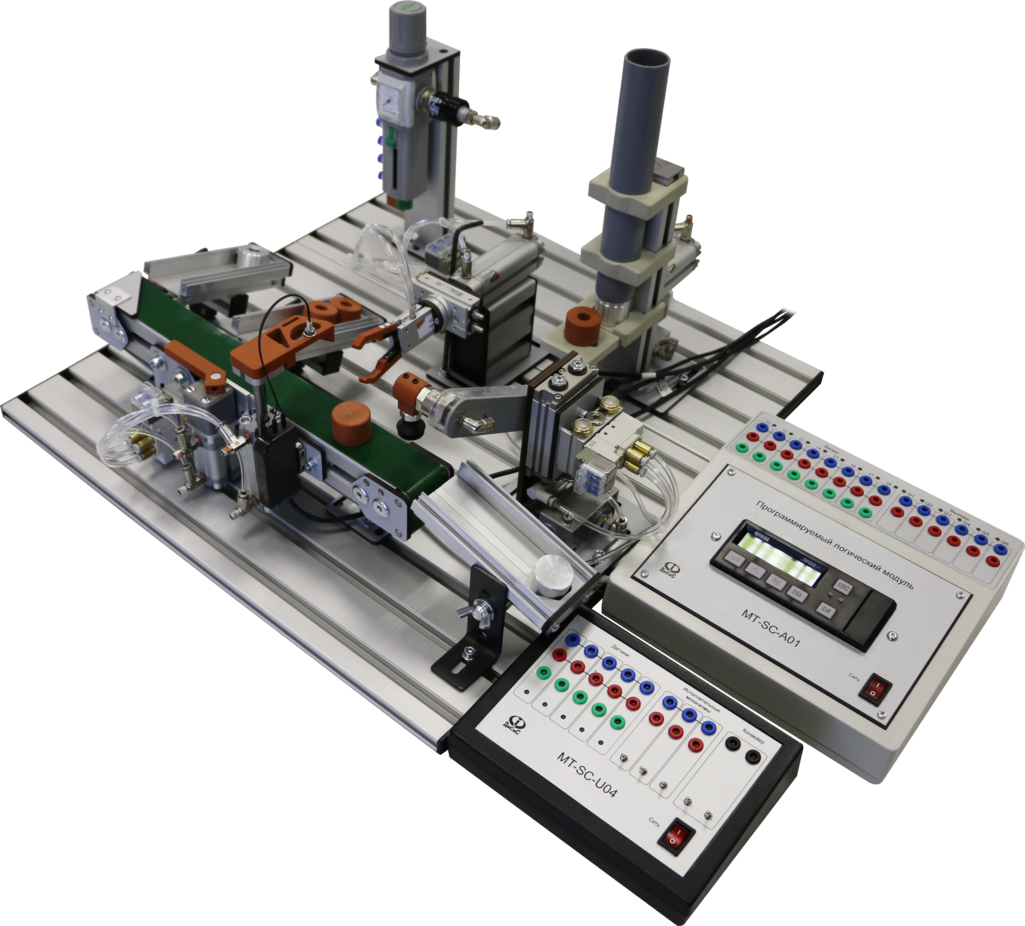
\includegraphics[scale=0.30]{fig/3.1.png}
    \caption{Комплект <<Основы мехатроники>> модели DISYS МТ-SС-1}
    \label{fig:all}
\end{figure}

\section{Комплектность}
\begin{itemize}
    \item Гравитационный магазин
    \item Пневматический перекладчик
    \item Пневматический манипулятор
    \item Ленточный конвейер
    \begin{itemize}
        \item Оптический датчик с разнесенной оптикой (1шт.)
        \item Оптоволоконный датчик (1шт.)
        \item Индуктивный датчик (1шт.)
    \end{itemize}
    \item Информационная платформа
    \begin{itemize}
        \item Оптоволоконный датчик (не менее 2 шт.)
        \item Индуктивный датчик
    \end{itemize}
    \item Приемный лоток (не менее 4 шт.)
    \item Блок подготовки воздуха
    \item Герконовый датчик положения (не менее 13 шт.)
    \item Модуль ручного управления (не менее 4 шт.)
    \item Программируемый логический модуль (не менее 2 шт.)
    \item Монтажная плита (не менее 4 шт.) размер одной плиты не менее\\(ШхДхВ), мм 180х500х15
    \item Набор деталей; (пластиковый цилиндр, пластиковый стакан, металлический цилиндр и металлический стакан.3 шт.каждого типа)
\end{itemize}

\section{Технические характеристики}
\begin{table}[hb]
    \centering
    \begin{tabular}{m{108mm}|l}
    Масса, не более, кг              & 10          \\
    Габаритные размеры, мм (ШхГхВ)   & 600x600x350 \\
    Напряжение питания, В/Гц         & 220/50      \\
    Рабочее напряжение, пост. ток, В & 24          \\
    Рабочее давление, МПа            & 0,4
    \end{tabular}
\end{table}

Условия эксплуатации компонентов набора - в помещении при температурах от + 10 до + 35° С и относительной влажности воздуха до 80 \% при 25° С.
\chapter{ОЗНАКОМЛЕНИЕ С ПРОГРАММНЫМ ОБЕСПЕЧЕНИЕМ}
OWEN Logic --- среда программирования, предназначенная для создания алгоритмов работы коммутационных приборов, программируемых логических контроллеров, относящихся к классу программируемых реле, в частности, приборов серий ПР1хх, ПР200 и панели ИПП120 производства компании ОВЕН. Программируемые логические контроллеры (далее ПЛК) -- это свободно программируемое устройство. Алгоритм работы ПЛК формируется непосредственно пользователем, что делает прибор универсальным и дает возможность широко использовать его в различных областях.

OWEN Logic позволяет пользователю разработать программу автоматизации системы по собственному алгоритму и записать ее в энергонезависимую память прибора. Для составления программы используется графический язык FBD, который применяется в цифровых электрических схемах. Также присутствует возможность создания блоков-макросов на языке ST или FBD.

Для работы OWEN Logic требуется операционная система Windows XP/7/8/10 и программная платформа «.NET Framework» версии 4.0. или выше.

\begin{figure}[hb]
    \centering
    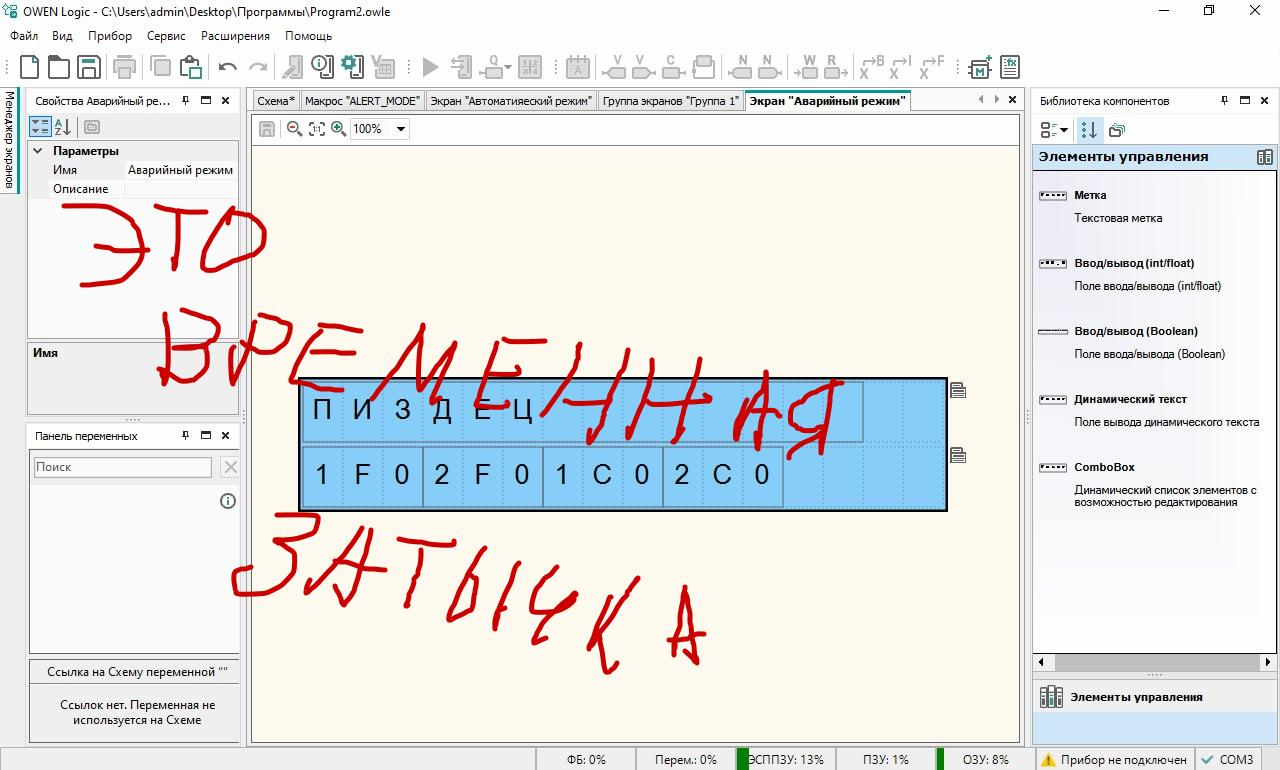
\includegraphics[scale=0.30]{fig/4.1.jpg}
    \caption{Интерфейс программы Owen Logic}
    \label{fig:owenlogic}
\end{figure}

\newpage
\section{Описание интерфейса}
Главное окно содержит:
\begin{itemize}
    \item Главное меню: Файл, Вид, Прибор, Сервис, Расширения, Помощь
    \item Панели инструментов
    \item Панели Библиотека компонентов, Свойства и Переменные (до открытия или создания проекта в них нет информации)
    \item Рабочую область проекта -- поле редактирования программы (до открытия или создания проекта пустое)
    \item Строку состояния в нижней части главного окна, показывающую информация о доступных ресурсах прибора и подключении к OWEN Logic
    \item Менеджер экранов
\end{itemize}

\section{Принцип выполнения программы}
Программа для прибора составляется с учетом количества имеющихся у него входов, выходов и наличия часов реального времени.

Работу прибора можно представить в виде последовательно выполняемых шагов (рабочий цикл):
\begin{enumerate}
    \item Логическое состояние входов автоматически записывается в ячейки памяти входов (количество ячеек равно числу входов -- I1\dots In).
    \item Программа считывает значения из ячеек памяти входов и выполняет над ними логические операции в соответствии с алгоритмом работы.
    \item После обработки всей программы результаты записываются на физические выходы прибора (для включения выходных элементов Q1\dots Q4).
    \item Переход к Шагу 1 (после выполнения всех предыдущих шагов обработки программы цикл работы прибора повторяется с первого шага).
\end{enumerate}
Время выполнения всех шагов зависит от сложности алгоритма программы.
\chapter{ВЫПОЛНЕНИЕ ЗАДАНИЯ}
Необходимо разработать программу для ПЛК для управления автоматизированной
установкой в соответствии с описанием ее работы.

\textbf{Цель} --- Сделать программу для управления автоматизированной установкой в соответствии с описанием ее работы.

При выполнении ставятся следующие задачи:
\begin{enumerate}
    \item Внимательно ознакомиться с заданием
    \item Изучить алгоритм работы установки
    \item Изучить электрическую схему подключения
    \item Изучить пневматическую схему подключения
    \item Определить сигналы для выполнения исполнительных элементов
    \item Создать программу для управления установкой
\end{enumerate}

Автоматическая установка состоит из трех пневматических цилиндров, шести
датчиков положения (герконы), одного двигателя постоянного тока и световой
колонны. Всеми перемещениями механизмов и индикацией световой колонны
управляет ПЛК (программируемый логический контроллер/программируемое
реле). Используется ПЛК ОВЕН ПР200-24 1.X.
Для реализации панели оператора используется встроенный scada система.

\section{Виртуальная панель оператора}
Виртуальная панель оператора в scada системе представлена на рисунке \ref{fig:scada_panel}.
\begin{figure}[hb]
    \centering
    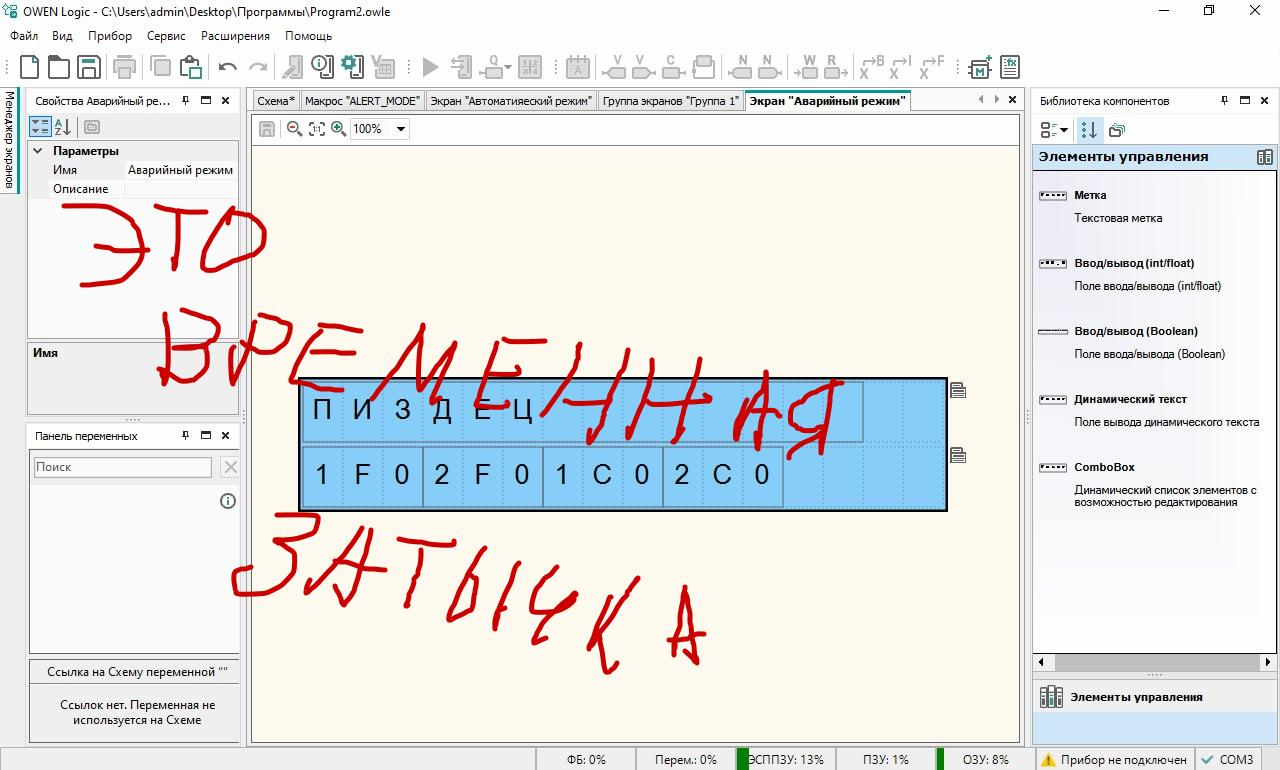
\includegraphics[scale=0.30]{fig/4.1.jpg}
    \caption{Виртуальная панель оператора}
    \label{fig:scada_panel}
\end{figure}

\subsection{Описание клавиш панели оператора}
\begin{enumerate}
    \item F1 -- аварийный останов (1 – активация)
    \item F2 -- ручной/авто (0 – ручной, 1 – автоматический)
    \item F3 -- старт (авто) / движение выбранного цилиндра (ручной)
    \item F4 -- движение выбранного цилиндра (ручной)
    \item С1 -- выбор цилиндра 1 (ручной)
    \item С2 -- выбор цилиндра 2 (ручной)
    \item С3 -- выбор цилиндра 3 (ручной)
    \item С4 -- включение двигателя (ручной)
\end{enumerate}

Из кнопок F1, F2, С1, С2, С3, С4 необходимо сделать переключатели
программным способом.

\section{Условия запуска установки}
\begin{itemize}
    \item Штекер вставлен в розетку и ручной пневматический клапан открыт для подачи воздуха в систему.
    \item Все компоненты должны оставаться в своих стартовых позициях, цилиндры 1, 2 и 3 втянуты, двигатель выключен.
    \item Выбор режима работы автоматический/ручной может быть осуществлен переключателем F2.
    \item Установка начинает свою работу только если кнопка аварийного останова F1 не активирована.
\end{itemize}




\chapter{УСТРАНЕНИЕ НЕИСПРАВНОСТЕЙ}
\begin{table}[h]
    \begin{tabular}{|m{50mm}|m{50mm}|m{50mm}|}
    \hline
    Неисправность                                                            & Возможные причины                                                                                                                                        & Устранение                                                                                                                                                               \\
    \hline
    Утечки воздуха в местах присоединения пневматических трубок к устройству & Трубка вставлена не до упора                                                                                                                             & Вставить трубку до упора                                                                                                                                                 \\
    \hline
    Не работает один из пневматических исполнительных механизмов             & Недостаточное давление сжатого воздуха в пневмосистеме\newline\newline Сдвинуты датчики, фиксирующие положение выходного звена & Настроить давление с помощью БПВ (давление на входе в БПВ должно быть не менее 4 бар)\newline\newline Установить датчики в требуемое положение \\
    \hline
    На информационной платформе оба оптических датчика работают одинаково    & Сбились настройки оптического датчика                                                                                                                    & Настроить работу одного датчика на фиксацию дна стакана, второго -- на фиксацию отверстия                                                                                \\
    \hline
    Детали не сползают в приемный лоток                                      & Нарушено взаимное расположение лотка и подающего механизма                                                                                               & Выставить лоток относительно механизма требуемым образом                                                                                                                \\
    \hline
    \end{tabular}
    \end{table}



%\textbf{Неисправность:} Утечки воздуха в местах присоединения пневматических трубок к устройству\\
%\textbf{Возможные причины:} Трубка вставлена не до упора\\
%\textbf{Устранение:} Вставить трубку до упора\\
%
%
%\textbf{Неисправность:} Не работает один из пневматических исполнительных механизмов\\
%\textbf{Возможные причины:}
%\begin{itemize}
%    \item Недостаточное давление сжатого воздуха в пневмосистеме
%    \item Сдвинуты датчики, фиксирующие положение выходного звена
%\end{itemize}
%\textbf{Устранение:}
%\begin{itemize}
%    \item Настроить давление с помощью БПВ (давление на входе в БПВ должно быть не менее 4 бар)
%    \item Установить датчики в требуемое положение
%\end{itemize}
%
%
%
%\textbf{Неисправность:} На информационной платформе оба оптических датчика работают одинаково
%\textbf{Возможные причины:} Сбились настройки оптического датчика
%\textbf{Устранение:} Настроить работу одного датчика на фиксацию дна стакана, второго -- на фиксацию отверстия
%
%
%
%\textbf{Неисправность:} Детали не сползают в приемный лоток
%\textbf{Возможные причины:} Нарушено взаимное расположение лотка и подающего механизма
%\textbf{Устранение:} Выставить лоток относительно механизма требуемым образом
%Заключение
\chapter*{ЗАКЛЮЧЕНИЕ}
\addcontentsline{toc}{chapter}{ЗАКЛЮЧЕНИЕ}

Во время прохождения учебной практики по профессиональному
модулю \module\ мною была реализована программа практики в полном
объёме. Общие и профессиональные компетенции по профессиональному
модулю получили развитие.

Прохождение практики прошло организованно, эффективно и, в целом,
оказало большую социальную значимость для моей будущей специальности.

Задание на практику выдано своевременно. На предприятии работали под
руководством руководителя практики. Был разработан технологический
процесс изготовления детали.
%Библиография
\renamebiblio
%настройка библиографии по ГОСТ
%\usepackage[
%    natbib		= true,
%    style		= gost-numeric,
%    sorting		= nyvt,
%    backend		= biber,
%    language	= autobib,
%    autolang	= other]{biblatex}

\begin{thebibliography}{2}
    \bibitem{1}
    \textbf{Paul Uttley} Robot Builder’s Guide for NI myRIO: учебное пособие / Professor R. H. Bishop; University of South Florida -  South Florida: Pitsco, Inc. -- 2015 г..
    \bibitem{2}
    \textbf{Аарон Локк} Методическое пособие к набору TETRIX: учебное пособие / Памела Сайферс, Тим Лэнкфорд; Университет Южной Флориды - Южная Флорида: Pitsco, Inc. -- 2018 г..
    \bibitem{3}
    \textbf{Пол Аттли} Робототехнический набор TETRIX руководство по сборке: учебное пособие / Невин Джонс, Аарон Локк; Университет Южной Флориды - Южная Флорида: Pitsco, Inc. -- 2018 г..
\end{thebibliography}

\clearpage
\pagestyle{empty}
\newpage
%\chapter*{ДНЕВНИК ПРОХОЖДЕНИЯ УЧЕБНОЙ ПРАКТИКИ}
{\textbf{\normalsize\centering ДНЕВНИК ПРОХОЖДЕНИЯ УЧЕБНОЙ ПРАКТИКИ}}
\begin{center}
\begin{tabular}{|l|m{100mm}|m{27mm}|}
    \hline
    Дата & Содержание работ & Отметка о выполнении\\
    \hline
    15.12.2021 & Ознакомление с техникой безопасности при работе с конструктором & \\
    \hline
    16.12.2021 & Ознакомление с техникой безопасности при работе с электрооборудованием & \\
    \hline
    17.12.2021 & Ознакомление с набором Tetrix Prime & \\
    \hline
    19.12.2021 & Сборка робота \textnumero 1 по инструкции & \\
    \hline
    20.12.2021 & Подключение электрооборудования и испытание робота \textnumero 1 & \\
    \hline
    21.12.2021 & Сборка робота \textnumero 2 по инструкции & \\
    \hline
    22.12.2021 & Подключение электрооборудования и испытание робота \textnumero 2 & \\
    \hline
    23.12.2021 & Сборка робота \textnumero 3 по инструкции & \\
    \hline
    24.12.2021 & Подключение электрооборудования и испытание робота \textnumero 3 & \\
    \hline
    26.12.2021 & Самостоятельная сборка робота в соответствии с заданием & \\
    \hline
    27.12.2021 & Подключение электрооборудования и испытание самостоятельно собранного робота & \\
    \hline
    28.12.2021 & Сдача дифф. зачета & \\
    \hline
\end{tabular}\\[\bigskipamount]

Руководитель практики\ \hrulefill\ \fullmaster\\
{\scriptsize Подпись}\\[\bigskipamount]

Дата \hbox to 5cm{\hrulefill}

\end{center}
\end{document}